%!TEX root = ../slides.tex
\section{State of the art}
\subsection{Mobile Sensing Apps}
\begin{frame}{State of the art}{Taxonomy of solutions}
\begin{figure}
  \centering
  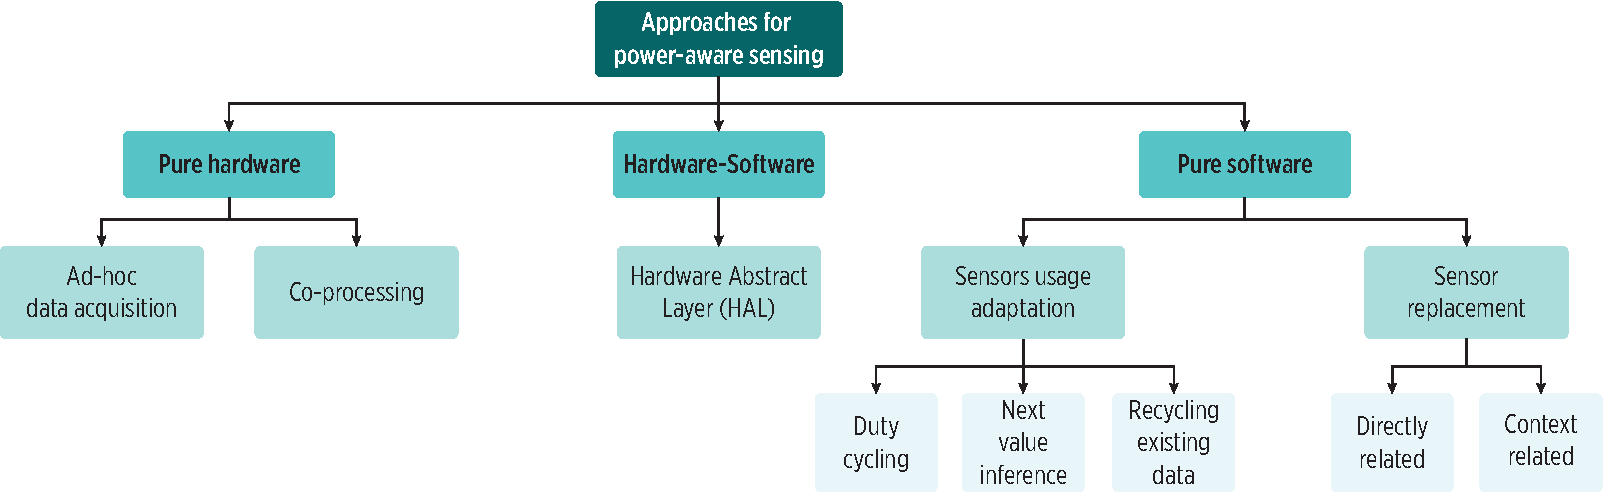
\includegraphics[width=0.9\textwidth]{vectors/approaches-taxonomy-for-slides}
  \caption{Taxonomy of solutions for power-aware sensing in mobility sensing systems.}
\end{figure}
\end{frame}

\subsection{Remarks}
\begin{frame}{State of the art}{Remarks}
\small
\begin{block}{\small \textbf{Remarks}}
\begin{itemize}
  \item The exploitation of coarse and fine-grain mobility information for modeling and characterizing user mobility has been barely explored.
  \item Although some of the proposed solutions employ a duty cycling strategy, it is fixed and obeys to instant mobility information, neglecting the temporal evolution of user mobility.
  \item A spatial-time accurate and energy efficient adaptive sampling could be produced by a cognitive approach that understands long-term mobility from fine and coarse-grain mobility events.
  \item The cognitive approach goes beyond typical pattern recognition and classic control strategies that follow a static configuration, as it evolves (in the learning and action tasks) across time.
  \item The smartphone itself could augment not only its location but also its mobility awareness (per-user basis).
\end{itemize}
\end{block}
\end{frame}